\section{Espelho de Corrente}
\label{anexoespelhos}

\subsection{Espelho de Corrente NMOS}

Um espelho de corrente \'e um circuito que replica o sinal de uma corrente de refer\^encia em outras sa\'idas, podendo ser multiplicado por um fator de ajuste. A \autoref{fig_espelho} mostra a representa{\c c}\~ao de um circuito com tal caracter\'istica, utilizando transistores NMOS. O espelho de corrente NMOS tamb\'em \'e chamado de dreno de corrente, por drenar a corrente nos ramos.

\begin{figure}[htb]
    \label{fig_espelho}
    \centering
    \caption{Espelho de corrente NMOS} 
    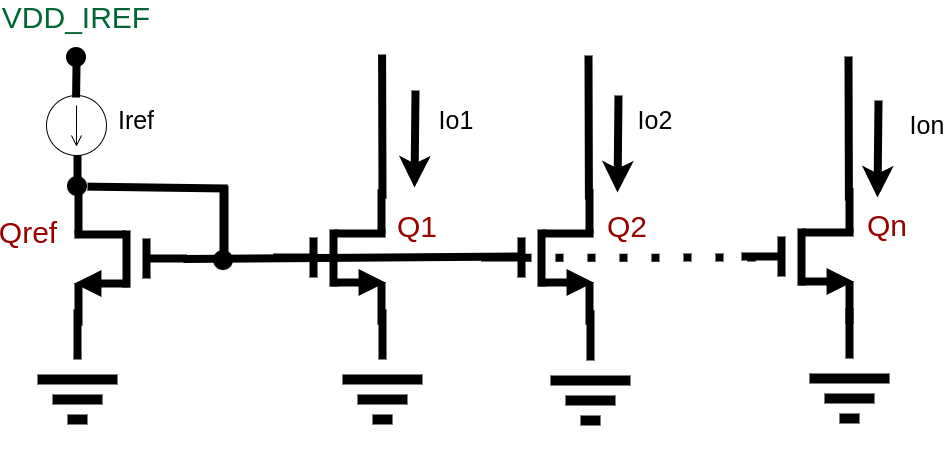
\includegraphics[scale=0.4]{Circuitos/current_mirror_example.png}
    \legend{Fonte: Produzido pelo autor}
\end{figure}

Nesta figura, est\'a representado a utiliza{\c c}\~ao de uma corrente de refer\^encia Iref para gerar as correntes Io1, Io2 at\'e Ion, onde "n" \'e o n\'umero de transistores se referenciando por \emph{Qref}.

No circuito demonstrado pela \autoref{fig_espelho}, o transistor \emph{Qref} tem func\^ao de captar a corrente igual \'a \emph{Iref}, para servir de refer\^encia aos outros transistores \emph{Q1}, \emph{Q2} at\'e \emph{Qn}, onde \emph{n} \'e o numero de transistores que se referenciam de \emph{Qref}, e que s\~ao chamados de bra{\c c}os do espelho. O potencial \emph{VDD\_IREF} \'e um valor de tens\~o utilizado para polarizar Iref, que n\~ao precisa ser igual ao valor de alimenta{\c c}\~ao dos outros bra{\c c}os.

Dado os parâmetrosWx/Lnde cada transistor, onde "x" é o número indicado do transistor, podemos calcular o valor de corrente de cada braço utilizando a fórmula apresentada na \autoref{eq_espcorpmos}.

\begin{equation}
    \label{eq_espcor}
    I_{OX} = Iref\frac{W_x/L_x}{W_{ref}/L_{ref}}
\end{equation}

Onde $I{ox}$ \'e a corrente de entrada do bra{\c c}o \emph{Qx}. 

Para que esse circuito funcione devidamente em cada sa\'ida, cada bra{\c c}o do espelho deve estar necessariamente operando na regi\~ao ativa, pois a \autoref{eq_espcor} \'e deduzida levando isso em conta. Para que isso aconte{\c c}a, devemos respeitar a \autoref{eq_curmirror_req} \cite{RazaviFundM}.

\begin{equation}
    \label{eq_curmirror_req}
    v_{DS} \geq v_{GS} - V_t
\end{equation}

Onde:

\begin{itemize}
    \item $v_{DS}$ \'e a tens\~ao entre o dreno e fonte do transistor
    \item $v_{GS}$ \'e a tens\~ao entre o porta e fonte do transistor
    \item $V_{t}$ \'e a tens\~ao de limiar do transistor
\end{itemize}

\subsection{Espelho de Corrente PMOS}

Um circuito de espelho de corrente pode ser constru\'ido com transistores PMOS, utilizando o mesmo racioc\'inio de constru{\c c}\~ao do circuito NMOS, conforme a \autoref{fig_curmir_pmos}. A diferen{\c c}a principal \'e que em vez de ser um dreno de corrente, o PMOS ser\'a um fornecedor de corrente.

\begin{figure}[htb]
    \label{fig_cur}
    \centering
    \caption{Espelho de corrente PMOS} 
    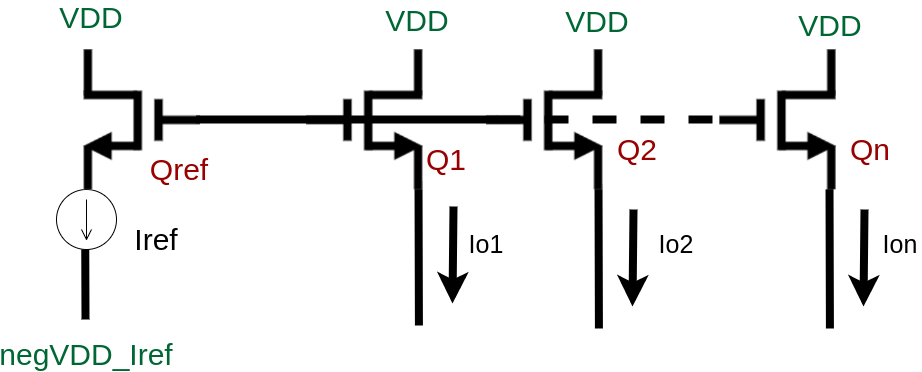
\includegraphics[scale=0.4]{Circuitos/current_mirror_example_pmos.png}
    \legend{Fonte: Produzido pelo autor}
\end{figure}

O funcionamento do circuito PMOS segue o mesmo principio do NMOS, porém, ao inv\'es de receber corrente fixada a um n\'o, ele fornece. O potencial \emph{negVDD\_IREF} \'e um valor de tens\~o utilizado para polarizar Iref, que n\~ao precisa ser igual ao valor de alimenta{\c c}\~ao negativa/terra dos outros bra{\c c}os.

Dado os parâmetrosWx/Lnde cada transistor, onde "x" é o número indicado do transistor, podemos calcular o valor de corrente de cada braço utilizando a fórmula apresentada na \autoref{eq_espcorpmos}.

\begin{equation}
    \label{eq_espcorpmos}
    I_{OX} = I_{ref}\frac{W_x/L_x}{W_{ref}/L_{ref}}
\end{equation}

Onde $I_{OX}$ \'e a corrente de sa\'ida do bra{\c c}o \emph{Qx}. 

Assim como no caso do NMOS, todos transistores devem estar na regi\~ao ativa, e respeitar a seguinte \autoref{eq_curmirror_reqpmos} \cite{RazaviFundM}.

\begin{equation}
    \label{eq_curmirror_reqpmos}
    v_{SD} \geq v_{SG} - |V_t|
\end{equation}

Onde:

\begin{itemize}
    \item $v_{SD}$ \'e a tens\~ao entre o fonte e dreno do transistor
    \item $v_{SG}$ \'e a tens\~ao entre a fonte e oirta do transistor
    \item $V_{t}$ \'e a tens\~ao de limiar do transistor
\end{itemize}

